\documentclass{article}

\usepackage[margin=1in]{geometry}
\usepackage{parskip}
\usepackage{graphicx}

\usepackage{tikz}

% from https://tex.stackexchange.com/a/36607/207458
\newcommand{\AxisRotator}[1][rotate=0]{%
  \tikz [x=0.25cm,y=0.60cm,line width=.2ex,-stealth,#1] \draw (0,0) arc (-150:150:1 and 1);%
}


% from https://tex.stackexchange.com/a/21957/207458
\usetikzlibrary{decorations}

\pgfdeclaredecoration{triangle}{start}{
  \state{start}[width=0.99\pgfdecoratedinputsegmentremainingdistance,next state=up from center]
  {\pgfpathlineto{\pgfpointorigin}}
  \state{up from center}[next state=do nothing]
  {
    \pgfpathlineto{\pgfqpoint{\pgfdecoratedinputsegmentremainingdistance}{\pgfdecorationsegmentamplitude}}
    \pgfpathlineto{\pgfqpoint{\pgfdecoratedinputsegmentremainingdistance}{-\pgfdecorationsegmentamplitude}}
    \pgfpathlineto{\pgfpointdecoratedpathfirst}
  }
  \state{do nothing}[width=\pgfdecorationsegmentlength,next state=do nothing]{
    \pgfpathlineto{\pgfpointdecoratedinputsegmentfirst}
    \pgfpathmoveto{\pgfpointdecoratedinputsegmentlast}
  }
}

\tikzset{
  triangle path/.style={decoration={triangle,amplitude=#1}, decorate},
  triangle path/.default=1ex
}

\usepackage{listings}
\lstset{
  basicstyle=\ttfamily\small,
  breaklines=true,
  frame=single
}
\usepackage{physics}
\usepackage{amsmath}
\usepackage{amssymb}
\usepackage{hyperref}
\hypersetup{
  colorlinks=true,
  linkcolor=blue,
  filecolor=magenta,
  urlcolor=cyan,
  pdftitle={INTDER Manual},
  pdfpagemode=FullScreen,
}

\title{Rust INTDER Manual}
\date{}
\author{Brent R. Westbrook}

\begin{document}

\maketitle

INTDER is a program for performing coordinate transformations between
simple-/symmetry-internal coordinates and Cartesian coordinates. It was
originally written in Fortran by Wesley D. Allen and coworkers but has since
been translated to Rust by Brent R. Westbrook. This documentation corresponds to
the Rust version only.

\section{Internal Coordinates}
\label{sec:coords}

At their most basic, internal coordinates are those defined with reference to
other atoms in the same molecule (or system), as opposed to an external set of
axes or some other frame of reference. Simple examples of internal coordinates
are distances between pairs of atoms and angles between sets of three atoms. A
major benefit of using internal coordinates over an external coordinate system
like Cartesian coordinates is that internal coordinates require only 3$N-6$ (or
3$N-5$ for linear molecules) coordinates to describe a system fully since the 3
translational and 3 rotational degrees of freedom only have meaning in an
external reference frame. $N$ in this case is, of course, the number of atoms in
the system. Given the exponential scaling of the number of points required to
describe a quartic force field (QFF), or really any potential energy surface
(PES), with the number atoms, this difference of 6 coordinates can have a large
effect. As a result, using internal coordinates can lead to a substantial
decrease in computational cost for such a PES.

\subsection{Simple-Internal Coordinates}
\label{sec:simple}

Simple-internal coordinates are the basic building blocks of symmetry-internal
coordinates, the major focus of the rest of the manual. The types of
simple-internal coordinates supported by INTDER are described in the following
subsections.

\subsubsection{Stretch}
\label{sec:stretch}

The bond stretch, referred to as \verb|STRE| in the input file, is the distance
between two atoms, as shown in Fig.~\ref{fig:stre}. When the direction matters,
the distance is computed from atom \verb|A| to atom \verb|B|, using the equation
given in Eqn.~\ref{eq:stre}, where $a_i$ and $b_i$ represent the $i$th
components of the Cartesian coordinates of atoms \verb|A| and \verb|B|,
respectively.

\begin{figure}[ht]
  \centering
  \caption{A stretch}
  \label{fig:stre}

  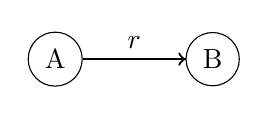
\begin{tikzpicture}
    \node[draw,circle] (A) at (0,0) {A};
    \node[draw,circle] (B) at (2,0) {B};
    \draw[thick, ->] (A) to (B);
    \draw[thick] (A) -- (B) node[midway, above] {$r$};
  \end{tikzpicture}
\end{figure}

\begin{equation}
  \label{eq:stre}
  r = \sqrt{\sum_i (b_i - a_i)^2}
\end{equation}

\subsubsection{Bend}
\label{sec:bend}

The bend, referred to as \verb|BEND| in the input file, is the angle between
three atoms, as shown in Fig.~\ref{fig:bend}.

\begin{figure}[ht]
  \centering
  \caption{A bend}
  \label{fig:bend}

  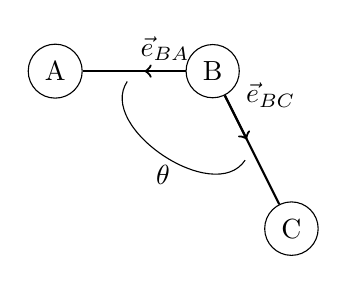
\begin{tikzpicture}
    \node[draw,circle] (A) at (0,0) {A};
    \node[draw,circle] (B) at (2,0) {B};
    \node[draw,circle] (C) at (3,-2) {C};
    \draw[thick] (A) -- (B) node[midway] (m) {};
    \draw[thick] (B) -- (C) node[midway] (n) {};
    \path (m) edge [bend left=-90] node[below] {$\theta$} (n);
    \draw[thick, ->] (B) -- (m) node[midway, above] {$\vec{e}_{BA}$};
    \draw[thick, ->] (B) -- (n) node[midway, above right] {$\vec{e}_{BC}$};
  \end{tikzpicture}
\end{figure}

The value of the angle, $\theta$ is computed using Eqn.~\ref{eq:bend}, where
$\vec{e}_{ij}$ represents the unit vector pointing from atom $i$ to atom $j$.

\begin{equation}
  \label{eq:bend}
  \theta = \acos(\vec{e}_{BA} \cdot \vec{e}_{BC})
\end{equation}

\subsubsection{Linear bend}
\label{sec:lin1}

The linear angle bend, referred to as \verb|LIN1| in the input file, is similar
to a regular bend, but atoms \verb|A|, \verb|B|, and \verb|C| are in a line, so
specifying the angle between them requires a fourth atom, \verb|D|, which must
be a dummy atom specified at the end of the geometry. Typically the coordinates
of \verb|D| are chosen to align with the central atom \verb|B| along the axis of
the molecule but to project along another axis, as shown in Fig.~\ref{fig:lin1}.

\begin{figure}[ht]
  \centering
  \caption{A linear bend}
  \label{fig:lin1}

  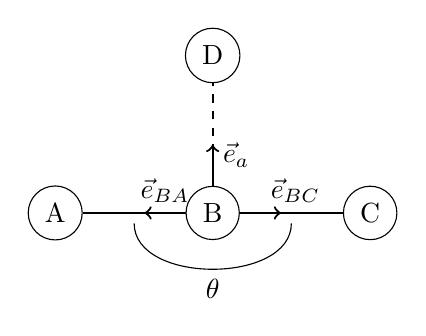
\begin{tikzpicture}
    \node[draw,circle] (A) at (0,0) {A};
    \node[draw,circle] (B) at (2,0) {B};
    \node[draw,circle] (C) at (4,0) {C};
    \node[draw,circle] (D) at (2,2) {D};
    \draw[thick] (A) -- (B) node[midway] (m) {};
    \draw[thick] (B) -- (C) node[midway] (n) {};
    \draw[thick, dashed] (B) -- (D) node[midway] (o) {};
    \path (m) edge [bend left=-90] node[below] {$\theta$} (n);
    \draw[thick, ->] (B) -- (m) node[midway, above] {$\vec{e}_{BA}$};
    \draw[thick, ->] (B) -- (n) node[midway, above right] {$\vec{e}_{BC}$};
    \draw[thick, ->] (B) -- (o) node[near end, right] {$\vec{e}_{a}$};
  \end{tikzpicture}
\end{figure}

The value of the linear bend is computed using Eqn.~\ref{eq:lin1} where
$\vec{e}_a$ is the unit vector in the Cartesian direction of the dummy atom.
Nothing in the code actually checks that it aligns with atom \verb|B|, so the
caller is responsible for making sure this is the case.

\begin{equation}
  \label{eq:lin1}
  \theta = \asin \big( \vec{e}_a \cdot (\vec{e}_{BC} \times \vec{e}_{BA}) \big)
\end{equation}

\subsubsection{Out}
\label{sec:out}

The out-of-plane bend, referred to as \verb|OUT| in the input file, is the angle
between atom \verb|A| and the plane formed by atoms \verb|B|, \verb|C|, and
\verb|D|, as shown in Fig.~\ref{fig:out}.

\begin{figure}[ht]
  \centering
  \caption{An out-of-plane bend}
  \label{fig:out}

  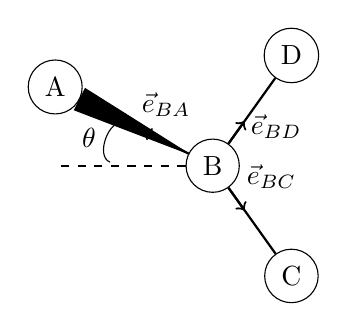
\begin{tikzpicture}
    \node[draw,circle] (A) at (0,1) {A};
    \node[draw,circle] (B) at (2,0) {B};
    \node[draw,circle] (C) at (3,-1.4) {C};
    \node[draw,circle] (D) at (3,1.4) {D};
    \draw[fill=black,triangle path] (B) -- (A) node[midway] (m) {};
    \draw[thick,dashed] (B) -- (0,0) node[midway] (s) {} ;
    \draw[thick] (B) -- (C) node[midway] (n) {};
    \draw[thick] (B) -- (D) node[midway] (o) {};
    \path (m) edge [bend left=-90] node[left] {$\theta$} (s);
    % \draw[thick, dashed] (B) -- (D) node[midway] (o) {};
    % \path (m) edge [bend left=-90] node[below] {$\theta$} (n);
    \draw[thick, ->] (B) -- (m) node[midway, above=.2cm] {$\vec{e}_{BA}$};
    \draw[thick, ->] (B) -- (n) node[midway, above right] {$\vec{e}_{BC}$};
    \draw[thick, ->] (B) -- (o) node[near end, right] {$\vec{e}_{BD}$};
  \end{tikzpicture}
\end{figure}

The value of $\theta$ is computed with the equations below, with the caveat that
if $w_1 + w_2$ is greater than zero, the value of theta is set to $\pi$ with the
sign of $\theta$, minus $\theta$.

\begin{align}
  \vec{v}_5 &= \vec{e}_{BC} \times \vec{e}_{BD} \\
  w_1 &= \vec{e}_{BA} \cdot \vec{e}_{BC} \\
  w_2 &= \vec{e}_{BA} \cdot \vec{e}_{BD} \\
  \phi &= \sin \big( \acos (\vec{e}_{BC} \cdot \vec{e}_{BD}) \big) \\
  \theta &= \asin ( \vec{e}_{BA} \cdot \vec{v}_5 / \phi)
\end{align}

\subsubsection{Torsion}
\label{sec:tors}

The torsional angle, referred to as \verb|TORS| in the input file, is the angle
between the planes formed by the overlapping sets of atoms \verb|A|, \verb|B|,
\verb|C|, and \verb|B|, \verb|C|, \verb|D|, as shown in Fig.~\ref{fig:tors}.
Vectors $\vec{v}_5$ and $\vec{v}_6$ are the vectors normal to the planes $ABC$
and $BCD$, respectively, found by $\vec{e}_{BA} \times \vec{e}_{CB}$ and
$\vec{e}_{DC} \times \vec{e}_{CB}$. To find the angle $\theta$ between these two
normals, and thus between the planes, perform the following transformations:

\begin{align}
  w_2 &= \vec{e}_{BA} \cdot \vec{e}_{CB} \\
  w_3 &= \vec{e}_{DC} \cdot \vec{e}_{CB} \\
  s_2 &= \sqrt{1 - w_2^2} \\
  s_3 &= \sqrt{1 - w_3^2} \\
  w_4 &= \vec{e}_{BA} \cdot \vec{v}_{6} \\
  w_5 &= -\vec{v}_5 \cdot \vec{v}_6 \\
  w &= \frac{w_2}{s_2 s_3} \\
  \theta_0 &= \asin w \\
  \theta &= \begin{cases}
              \theta_0 & w_3 \geq 0 \\
              \pi - \theta_0 & w_3 < 0
            \end{cases}
\end{align}

\begin{figure}[ht]
  \centering
  \caption{A torsion}
  \label{fig:tors}

  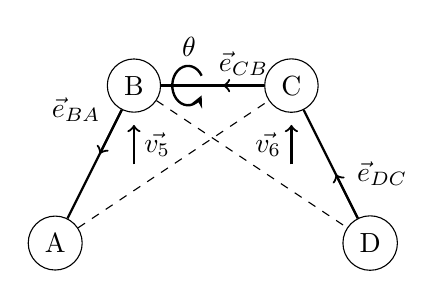
\begin{tikzpicture}
    \node[draw,circle] (B) at (0,0) {B};
    \node[draw,circle] (C) at (2,0) {C};
    \node[draw,circle] (D) at (3,-2) {D};
    \node[draw,circle] (A) at (-1,-2) {A};
    \draw[thick] (B) -- (A) node[midway] (m) {};
    \draw[thick] (C) -- (B) node[midway] (n) {};
    \draw[thick] (D) -- (C) node[midway] (o) {};
    \draw[thick, ->] (B) -- (m) node[midway, above left] {$\vec{e}_{BA}$};
    \draw[thick, ->] (C) -- (n) node[midway, above] {$\vec{e}_{CB}$};
    \draw[thick, ->] (D) -- (o) node[midway, above right] {$\vec{e}_{DC}$};
    % vectors
    \draw[thick, ->] (0,-1) -- (0,-0.5) node[midway, right] {$\vec{v_5}$};
    \draw[thick, ->] (2,-1) -- (2,-0.5) node[midway, left] {$\vec{v_6}$};
    % planes
    \draw[dashed] (A) -- (C);
    \draw[dashed] (B) -- (D);

    \draw (n) node [left] {\AxisRotator[x=0.2cm,y=0.25cm,rotate=180]};
    \draw (n) node [left=0.3cm, above=0.25cm] {$\theta$};
  \end{tikzpicture}
\end{figure}

\subsection{Symmetry-Internal Coordinates}
\label{sec:symm}

With a solid foundation in simple-internal coordinates, symmetry-internal
coordinates (SICs) require much less explanation. SICs are simply linear
combinations of simple-internal coordinates that can be treated as a single
unit. Common examples of SICs include the symmetric stretch in water, which is
the positive combination (sum) of the O-H$_1$ stretch and the O-H$_2$ stretch;
and the anti-symmetric stretch of water, which is the negative combination
(difference) of the two O-H stretches. In the case of water, the third SIC only
has a single component, the simple-internal bending coordinate. INTDER accepts
linear combinations of any number of simple-internal coordinates, but as you may
imagine, the generation of highly-symmetrical SIC systems becomes very
difficult. Describing how to approach such a problem is beyond the scope of this
manual, if not beyond the scope of its author's abilities. Such is the major
weakness of SICs in general.

\subsection{Input Format}
\label{sec:coord-inp}

The listing below shows an example of simple- and symmetry-internal coordinate
input for the formaldehyde (H$_2$CO) molecule, followed by the geometry to help
picture the meaning of these coordinates.

\begin{lstlisting}
STRE     1    2
STRE     2    3
STRE     2    4
BEND     1    2    3
BEND     1    2    4
OUT      1    2    3    4
    1   1   1.000000000
    2   2   1.000000000   3   1.000000000
    3   4   1.000000000   5   1.000000000
    4   2   1.000000000   3  -1.000000000
    5   4   1.000000000   5  -1.000000000
    6   6   1.000000000
    0
      0.000000000        0.000000000       -1.137981497
      0.000000000        0.000000000        1.140677167
      0.000000000        1.771466895        2.235424580
      0.000000000       -1.771466895        2.235424580
\end{lstlisting}

The first section defines the internal coordinates themselves, given in more
descriptive notation below and with atom labels corresponding to
Fig.~\ref{fig:h2co}. This format is straightforward: the name of the coordinate
occurs in the first column, followed by the number of the atom in the Cartesian
geometry that follows in the order described in the previous sections.

\begin{figure}[ht]
  \centering
  \caption{Simple-internal coordinates of formaldehyde}
  \label{fig:h2co}

  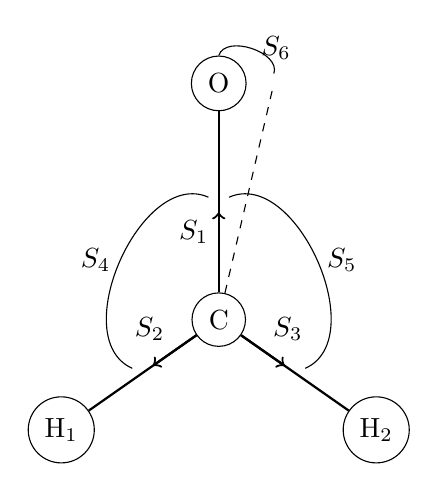
\begin{tikzpicture}
    \node[draw,circle] (A) at (0,-1.4) {H$_1$};
    \node[draw,circle] (B) at (2,0) {C};
    \node[draw,circle] (C) at (4,-1.4) {H$_2$};
    \node[draw,circle] (D) at (2,3) {O};
    \draw[thick] (A) -- (B) node[midway] (m) {};
    \draw[thick] (B) -- (C) node[midway] (n) {};
    \draw[thick] (B) -- (D) node[midway] (o) {};
    \path (m) edge [bend left=90] node[left] {$S_4$} (o);
    \path (n) edge [bend left=-90] node[right] {$S_5$} (o);
    \draw[thick, ->] (B) -- (m) node[midway, above left] {$S_2$};
    \draw[thick, ->] (B) -- (n) node[midway, above right] {$S_3$};
    \draw[thick, ->] (B) -- (o) node[near end, left] {$S_1$};

    \draw[dashed] (B) -- (2.7,3) node (x) {};
    \path (x) edge [bend left=-90] node[right] {$S_6$} (D);
  \end{tikzpicture}
\end{figure}

\begin{align}
  S_1 &= r(\text{O}-\text{C}) \\
  S_2 &= r(\text{C}-\text{H}_1) \\
  S_3 &= r(\text{C}-\text{H}_2) \\
  S_4 &= \angle(\text{O}-\text{C}-\text{H}_1) \\
  S_5 &= \angle(\text{O}-\text{C}-\text{H}_2) \\
  S_6 &= OUT(\text{O}-\text{CH}_2)
\end{align}

The second section defines the SICs as linear combinations of the
simple-internals. The first column represents the SIC number, every pair of
following columns represents a simple-internal coordinate and its coefficient.
In practice all of these coefficients are 1.0, so this format is likely to
change in the future. Positive coefficients, such as those for SIC 2 and SIC 3,
are symmetric coordinates like the symmetric stretch for water discussed
earlier. Similarly, negative coefficients, like the second components of SICs 4
and 5, correspond to anti-symmetric coordinates where one simple-internal
coordinate increases while the other decreases. An SIC number of 0 at the start
of the line signals the end of the SIC section.

SICs can also be written algebraically, as shown in the equations below. Note
also the normalization constant that must be applied to give the whole SIC a
magnitude of 1. This constant has the general form $\frac{\sqrt{N}}{N}$, where N
is the number of simple-internal components, although the value for $N=2$ is
typically written as $\frac{1}{\sqrt{2}}$, which does not emphasize this form.

\begin{align}
  L_1 &= r(\text{O}-\text{C}) \\
  L_2 &= \frac{1}{\sqrt{2}}[r(\text{C}-\text{H}_1) + r(\text{C}-\text{H}_1)]\\
  L_2 &= \frac{1}{\sqrt{2}}[\angle(\text{O}-\text{C}-\text{H}_1) + \angle(\text{O}-\text{C}-\text{H}_2)]\\
  L_2 &= \frac{1}{\sqrt{2}}[r(\text{C}-\text{H}_1) - r(\text{C}-\text{H}_1)]\\
  L_2 &= \frac{1}{\sqrt{2}}[\angle(\text{O}-\text{C}-\text{H}_1) - \angle(\text{O}-\text{C}-\text{H}_2)]\\
  L_6 &= OUT(\text{O}-\text{CH}_2)
\end{align}

As a final note, the example input contains exactly the right format for the
Fortran version of INTDER, but the Rust version is much more forgiving with
spacing and alignment. As long as whitespace separates the fields of each line,
the Rust version should parse it correctly.

\end{document}